\documentclass[10pt]{article}
\usepackage[ruled, linesnumbered]{algorithm2e}
\usepackage{Jan1, epsfig, subfigure, amssymb, multirow, algorithmic,amsmath}
\usepackage{latexsym,amssymb,epsfig,graphicx,subfigure,rotating,multirow,colortbl,xcolor,amsmath,algorithmic,booktabs,url}
\usepackage{accents}
\usepackage{subfig}
\textwidth 160mm
\textheight 215mm
\voffset 1mm
\oddsidemargin 1mm
\evensidemargin 1mm
\newtheorem{definition}{Definition}
\newtheorem{theorem}{Theorem}
\newtheorem{proposition}{Proposition}
\newtheorem{conjecture}{Conjecture}
\newtheorem{corollary}{Corollary}
\newtheorem{lemma}{Lemma}
\newtheorem{example}{Example}


\usepackage[english]{babel}
\usepackage{blindtext}


\title{Implementing LIQSS2}

\author{Anton de Villiers\thanks{HealthQ Technologies, Office 9, First Floor, The Woodmill Lifestyle, Vredenburg Road, Devon Valley,
Stellenbosch, 7600, South Africa}}

\renewcommand{\thefigure}{\arabic{section}.\arabic{figure}}
\renewcommand{\thetable}{\arabic{section}.\arabic{table}}
\begin{document}
\setcounter{page}{1}



\newcommand{\blokkie}{\hspace{.07cm}\Box\hspace{.07cm}}

%%%%% Set up the coloured tables %%%%%
\colorlet{tableheadcolor}{gray!25} % Table header colour = 25% gray
\colorlet{tablerowcolor}{gray!10} % Table row separator colour = 10% gray
\newcommand{\headcol}{\rowcolor{tableheadcolor}}
\newcommand{\rowcol}{\rowcolor{tablerowcolor}}

% The top-most line of a table
\newcommand{\topline}{\arrayrulecolor{black}\specialrule{0.1em}{\abovetopsep}{0pt}%
	\arrayrulecolor{tableheadcolor}\specialrule{\belowrulesep}{0pt}{0pt}%
	\arrayrulecolor{black}}

	% The top-most line of a table
\newcommand{\toplinee}{\arrayrulecolor{black}\specialrule{0.1em}{\abovetopsep}{0pt}%
	\arrayrulecolor{tablerowcolor}\specialrule{\belowrulesep}{0pt}{0pt}%
	\arrayrulecolor{black}}

% The line between the headings and the table body
\newcommand{\midline}{\arrayrulecolor{tableheadcolor}\specialrule{\aboverulesep}{0pt}{0pt}%
	\arrayrulecolor{black}\specialrule{\lightrulewidth}{0pt}{0pt}%
	\arrayrulecolor{white}\specialrule{\belowrulesep}{0pt}{0pt}%
	\arrayrulecolor{black}}

% A line for when the upper row is rowcolor and the next line is white
\newcommand{\midlinecbw}{\arrayrulecolor{tablerowcolor}\specialrule{\aboverulesep}{0pt}{0pt}%
	\arrayrulecolor{black}\specialrule{\lightrulewidth}{0pt}{0pt}%
 	\arrayrulecolor{white}\specialrule{\belowrulesep}{0pt}{0pt}%
	\arrayrulecolor{black}}

% A line with no black, to further separate a rowcolor row and a white row
\newcommand{\midlinecw}{\arrayrulecolor{tablerowcolor}\specialrule{\aboverulesep}{0pt}{0pt}%
	\arrayrulecolor{tablerowcolor}\specialrule{\lightrulewidth}{0pt}{0pt}%
	\arrayrulecolor{white}\specialrule{\belowrulesep}{0pt}{0pt}%
	\arrayrulecolor{black}}

% A line for when the upper row is white and the next line is rowcolor
\newcommand{\midlinewbc}{\arrayrulecolor{white}\specialrule{\aboverulesep}{0pt}{0pt}%
	\arrayrulecolor{black}\specialrule{\lightrulewidth}{0pt}{0pt}%
	\arrayrulecolor{tablerowcolor}\specialrule{\belowrulesep}{0pt}{0pt}%
	\arrayrulecolor{black}}

% sadfsdfsdf sdfsdfsdf
\newcommand{\midlinehr}{\arrayrulecolor{tablerowcolor}\specialrule{\aboverulesep}{0pt}{0pt}%
	\arrayrulecolor{black}\specialrule{\lightrulewidth}{0pt}{0pt}%
	\arrayrulecolor{tableheadcolor}\specialrule{\belowrulesep}{0pt}{0pt}%
	\arrayrulecolor{tablerowcolor}}


% A line for the bottom of the table, when the last row is white
\newcommand{\bottomline}{\arrayrulecolor{white}\specialrule{\aboverulesep}{0pt}{0pt}%
	\arrayrulecolor{black}\specialrule{\heavyrulewidth}{0pt}{\belowbottomsep}}%

% A line for the bottom of the table, when the last row is rowcolor
\newcommand{\bottomlinec}{\arrayrulecolor{tablerowcolor}\specialrule{\aboverulesep}{0pt}{0pt}%
	\arrayrulecolor{black}\specialrule{\heavyrulewidth}{0pt}{\belowbottomsep}}%

\newcommand{\bottomlinect}{\arrayrulecolor{tableheadcolor}\specialrule{\aboverulesep}{0pt}{0pt}%
	\arrayrulecolor{black}\specialrule{\heavyrulewidth}{0pt}{\belowbottomsep}}%
%%%%% Set up the coloured tables %%%%%



\maketitle



\pagestyle{myheadings}

\section{Introduction}

The aim of this document is to provide a step-by-step numerical walk-through of the {\em second order} Linearly Implicit Quantised State Systems (LIQSS). Mogoni {\em et al.}~\cite{MigoniBortolottoKofmanCellier2013} provides an algorithm for calculating the $n$-th order LIQSS algorithm in general. This algorithm does not provide all the numerical calculations and intricacies required when implementing the solver on an actual ODE model.

In this document we will consider the Lotka-Volterra model. The Lotka-Volterra equations, also known as the predator-prey equations, are a pair of first-order, non-linear, differential equations frequently used to describe the dynamics of biological systems in which two species interact, one as a predator and the other as prey. The populations change through time according to the pair of equations:

\begin{align*}
\frac{dx_1(t)}{dt}  = \alpha x_1(t) - \beta x_1(t) x_2(t) \\[6pt]
\frac{dx_2(t)}{dt}  = \delta x_1(t) x_2(t)  - \gamma x_2(t)
\end{align*}

In this model $x_1(t)$ denotes the number of prey and $x_2(t)$ denotes the number of predators at time $t$. In this model we set the parameters as follows: $\alpha = \beta = \delta =0.5$ and $\gamma=0.3$.

QSS Solver\footnote{QSS Solver is an application that contains a family of QSS implemented solvers for addressing ODE systems.}~\cite{qss} is a modeling and simulation environment for continuous and hybrid systems. This simulation tool describe models using a subset of the Modelica language called MicroModelica~\cite{micro}. QSS Solver supports the entire family of QSS related solvers, including a family of Linearly Implicit QSS (LIQSS)~\cite{MigoniKofman2009} solvers which were created to deal with stiff mathematical systems.

When solving the Lotka-Volterra model for 100 seconds we obtain the numerical results displayed graphically in Figure~\ref{fig1}.

\begin{figure}[htbp]
\begin{center}
		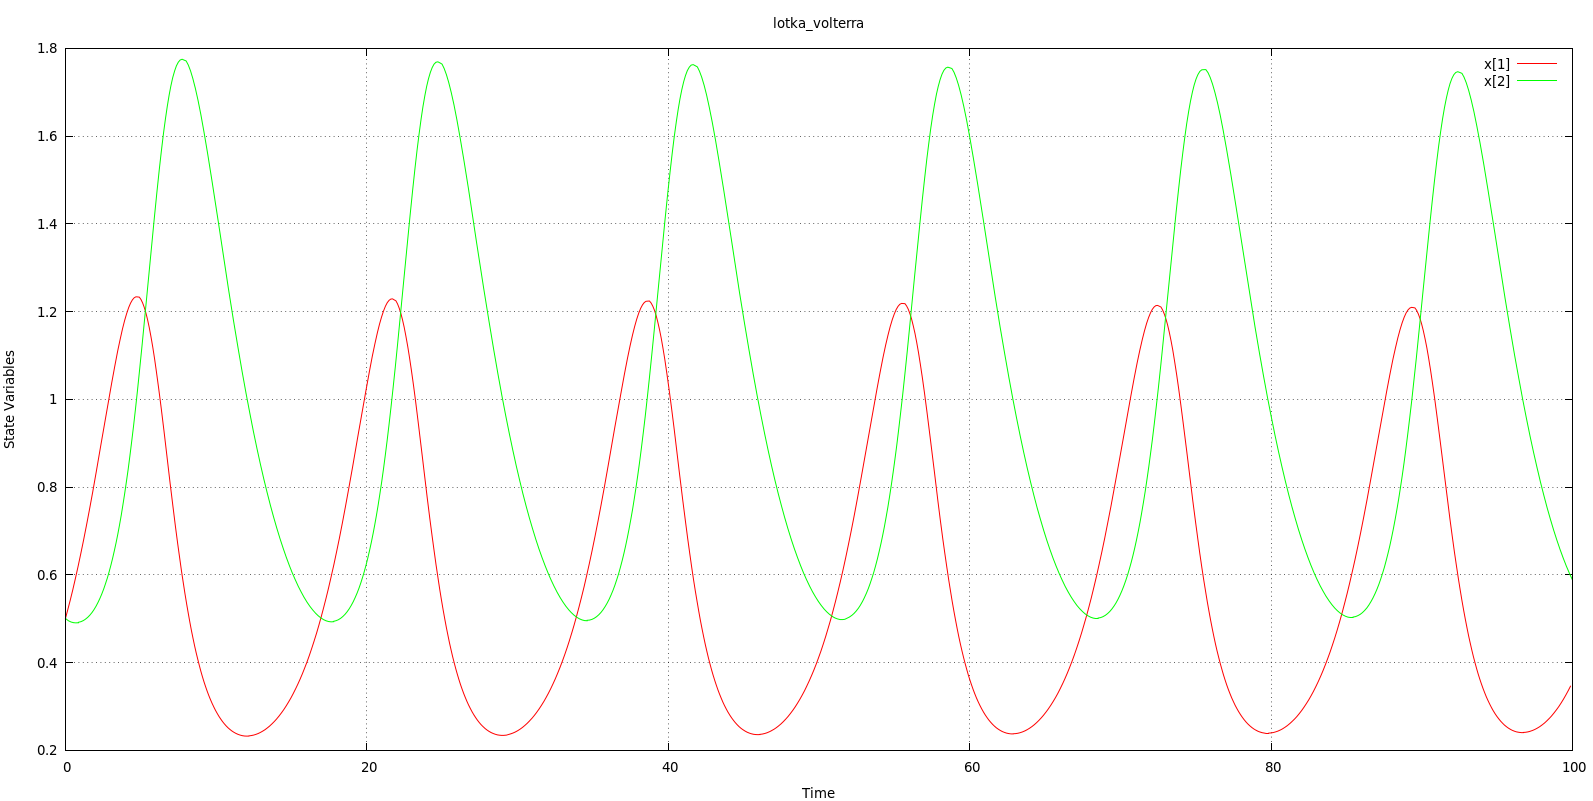
\includegraphics[scale=0.25]{./Figures/Selection_116.png}

\end{center}
\vspace{-0.5cm}

\caption{The Lotka-Volterra model simulated for 100 seconds.}\label{fig1}
\end{figure}



The rest of this document will consider the numerical implementation of the Lotka-Volterra model using the second order LIQSS solver in the QSS Solver application. Mogoni {\em et al.}~\cite{MigoniBortolottoKofmanCellier2013} provides an 8 step recursive algorithm to numerically solve an ODE for an $n$-th order LIQSS solver in general.

This document will not consider event handling within QSS Solver at all, since the Lotka-Volterra model does not contain any events.

\section{The second order derivatives}

QSS Solver makes use of GiNaC~\cite{ginac} to symbolically differentiate a system. Our first order derivatives look as follow:

\begin{align}
\dot{x}_1(t)  = 0.5 x_1(t) - 0.5 x_1(t) x_2(t) \label{W1}\\[6pt]
\dot{x}_2(t)  = 0.5 x_1(t) x_2(t)  - 0.3 x_2(t)\label{W2}
\end{align}

Using the product rule, our second order derivatives are as follow:

\begin{align}
\ddot{x}_1(t)  = 0.5 \dot{x}_1(t) - 0.5\left[ \dot{x}_1(t)x_2(t) + x_1(t)\dot{x}_2(t)\right]\label{W3} \\[6pt]
\ddot{x}_2(t)  = 0.5\left[ \dot{x}_1(t)x_2(t) + x_1(t)\dot{x}_2(t)\right]  - 0.3 \dot{x}_2(t) \label{W4}
\end{align}

\section{The actual code of QSS Solver}

QSS Solver has a very specific means of communicating with models that are created. Figure~\ref{fig2} displays the content of the root {\tt{qss-svoler}} directory.

\begin{figure}[htbp]
\begin{center}
		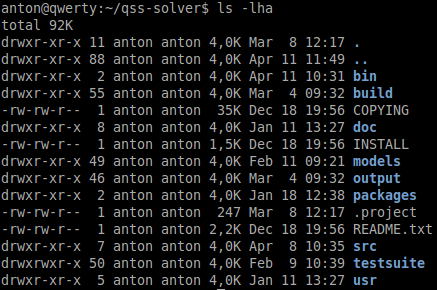
\includegraphics[scale=0.5]{./Figures/Selection_117.png}
\end{center}
\vspace{-0.5cm}

\caption{The root of {\tt{qss-solver}}.}\label{fig2}
\end{figure}

The most important (and relevant) subdirectories are:
\begin{itemize}
 \item {\tt{src}} --- containing all the code for solving the ODE models
  \item {\tt{models}} --- contains the {\tt{.mo}} files describing the model
   \item {\tt{build}} --- the converted model {\sf{C}} code is found here with some scripts
    \item {\tt{output}} --- the outputs of the most recent simulation run with {\tt{.dat}} data files.
\end{itemize}

To understand the workings of the solver we will investigate {\tt{src}} in much detail. To start we will provide a detailed flow of how the solver iterates over the various functions and methods during each iteration (time step) when solving a model.

\begin{table}[htbp]
	\centering\footnotesize
		\begin{tabular}{llp{5.5cm}}
    \topline	\headcol
    Function&Location& Description\\\midline
     \sf{QSS\_initSimulator}& {\tt{/engine/qss/qss-simulator.c}}&Initiates the simulation model. \\\rowcol
     \sf{QSS\_Simulator}& {\tt{/engine/qss/qss-simulator.c}}& Allocates memory, default values, {\em etc.}\\
     \sf{SIM\_simulate}&{\tt{/engine/common/qss-simulator.c}}& Initializes the simulator.\\\rowcol
     \sf{QSS\_simulate}&{\tt{/engine/qss/qss-simulator.c}} & Simulate the model.\\
     $\hookrightarrow$\sf{Random}&{\tt{/engine/common/random.c}} & Not sure what happen here.\\\rowcol
     $\hookrightarrow$\sf{getTime}& {\tt{/engine/common/utils.c}}& Retrieves CPU time.\\
     $\hookrightarrow${\sf{QSS\_initializeDataStructs}}& {\tt{/build/lotka\_volterra/lotka\_vol.c}}&Assigns values to the solver.\\\rowcol
     $\hookrightarrow${\sf{subTime}}& {\tt{/engine/common/utils.c}}& Computes difference between two CPU times.\\
     $\hookrightarrow${\sf{INT\_initialize}}&{\tt{/engine/common/integrator.c}}&Calls {\sf{QSS\_SEC\_initialize}}.\\\rowcol
     $\hookrightarrow$$\hookrightarrow${\sf{QSS\_SEC\_initialize}}&{\tt{/engine/qss/qss-integrator.c}}&Performs the initial values of derivatives and calculation related to initial variable settings.\\
     $\hookrightarrow$$\hookrightarrow${\sf{FRW\_recomputeDerivative}}&{\tt{/engine/qss/qss\_frw.c}}&Calls {\sf{SYM\_recomputeDerivative}}.\\\rowcol
     $\hookrightarrow$$\hookrightarrow${\sf{SYM\_recomputeDerivative}}&{\tt{/engine/qss/qss\_frw\_imp.c}}& Determines the derivatives.\\
     $\hookrightarrow$$\hookrightarrow${\sf{advanceTime}}&{\tt{/engine/common/utils.c}}& Determines the next time.\\\rowcol
     $\hookrightarrow$$\hookrightarrow${\sf{FRW\_nextInputTime}}&{\tt{/engine/qss/qss\_integrator.c}}& Calls {\sf{SO\_nextInputTime}}.\\
     $\hookrightarrow$$\hookrightarrow${\sf{SO\_nextInputTime}}&{\tt{/engine/qss/qss\_frw\_imp.c}}& Calculates next time based on \S4.3 in \cite{MigoniBortolottoKofmanCellier2013}\\\rowcol
     $\hookrightarrow$$\hookrightarrow${\sf{FRW\_nextEventTime}}&{\tt{/engine/qss/qss-integrator.c}}& Ignored for now\ldots\\
     $\hookrightarrow$$\hookrightarrow${\sf{QA\_recomputeNextTime}}&{\tt{/engine/qss/qss\_quantizer.c}}& Redirects call\\\rowcol
     $\hookrightarrow$$\hookrightarrow${\sf{LIQSS2\_recomputeNextTime}}&{\tt{/engine/qss/liqss2.c}}& Computes the next time step.\\
     $\hookrightarrow$$\hookrightarrow$$\hookrightarrow${\sf{minRootPos}}&{\tt{/engine/common/utils.c}}&Find smallest positive root in polynomial.\\\rowcol
     $\hookrightarrow$$\hookrightarrow${\sf{SC\_Scheduler}}&{\tt{/engine/qss/qss\_scheduler.c}}&Not entirely sure what happens here.\\
     $\hookrightarrow$$\hookrightarrow${\sf{getTimeValue}}&{\tt{/engine/qss/utils.c}}&Retrieves time from CPU.\\\rowcol
     $\hookrightarrow${\sf{QSS\_SEQC\_integrator.c}}&{\tt{/engine/qss/qss\_seqc\_integrator.c}}&Iteratively simulates all the time steps.\\
     $\hookrightarrow$$\hookrightarrow${\sf{advanceTime}}&{\tt{/engine/common/utils.c}}& Determines the next time.\\\rowcol
     $\hookrightarrow$$\hookrightarrow${\sf{QA\_updateQuantizedState}}&{\tt{/engine/qss/liqss2.c}}&Updates the $q$'s.\\
     $\hookrightarrow$$\hookrightarrow${\sf{QA\_nextTime}}&{\tt{/engine/qss/liqss2.c}}&Recalculates the derivatives\\\rowcol
     $\hookrightarrow$$\hookrightarrow${\sf{evaluatePoly}}&{\tt{/engine/common/utils.c}}&Finds value of a polynomial with input values.\\
     $\hookrightarrow$$\hookrightarrow${\sf{FRW\_recomputeDerivatives}}&{\tt{/engine/qss/qss\_frw.c}}&Calls {\sf{SYM\_recomputeDerivative}}\\\rowcol
     $\hookrightarrow$$\hookrightarrow$$\hookrightarrow${\sf{SYM\_recomputeDerivative}}&{\tt{/engine/qss/qss\_frw\_imp.c}}&Calculates the ODEs\\
     $\hookrightarrow$$\hookrightarrow${\sf{QA\_recomputeNextTime}}&{\tt{/engine/qss/liqss2.c}}& Computes next time\\\bottomline
    \end{tabular}
\caption{A basic layout of the function calls to simulate a model (in this case the Lotka-Volterra model) in QSS Solver with the LIQSS2 solver.}
\label{tab1}
    \end{table}

\section{The notation related to the variables}

Some of these variable alignments are specifically due for the Lotka-Volterra model.
\begin{table}[htbp]
	\centering\footnotesize
		\begin{tabular}{lllp{3.5cm}}
    \topline	\headcol
    Variable & Notation &Location& Description\\\midline
    {\tt{der[1]}}& $\dot{x}_1(t)$& {\sf{lotka\_volterra.c}}& Calculates of $\dot{x}_1$ at $t$.\\\rowcol
    {\tt{der[2]}}& $\ddot{x}_1(t)$& {\sf{lotka\_volterra.c}}& Calculates of $\ddot{x}_1$ at $t$.\\
    {\tt{der[4]}}& $\dot{x}_2(t)$& {\sf{lotka\_volterra.c}}& Calculates of $\dot{x}_2$ at $t$.\\\rowcol
    {\tt{der[5]}}& $\ddot{x}_2(t)$& {\sf{lotka\_volterra.c}}& Calculates of $\ddot{x}_2$ at $t$.\\
    {\tt{x[0]}}& $x_1(t)$& {\sf{qss\_integrator.c}}& Value of $x_1$ at $t$.\\\rowcol
    {\tt{x[1]}}& $\dot{x}_1(t)$& {\sf{qss\_integrator.c}}& Value of $\dot{x}_1$ at $t$.\\
    {\tt{x[2]}}& $\ddot{x}_1(t)$& {\sf{qss\_integrator.c}}& Value of $\ddot{x}_1$ at $t$.\\\rowcol
    {\tt{x[3]}}& $x_2(t)$& {\sf{qss\_integrator.c}}& Value of $x_2$ at $t$.\\
    {\tt{x[4]}}& $\dot{x}_2(t)$& {\sf{qss\_integrator.c}}& Value of $\dot{x}_2$ at $t$.\\\rowcol
    {\tt{x[5]}}& $\ddot{x}_2(t)$& {\sf{qss\_integrator.c}}& Value of $\ddot{x}_2$ at $t$.\\
    {\tt{q[0]}}& $q_1(t)$& {\sf{qss\_integrator.c}}& Value of $q_1$ at $t$.\\\rowcol
    {\tt{q[1]}}& $\dot{q}_1(t)$& {\sf{qss\_integrator.c}}& Value of $\dot{q}_1$ at $t$.\\
    {\tt{q[2]}}& $\ddot{q}_1(t)$& {\sf{qss\_integrator.c}}& Value of $\ddot{q}_1$ at $t$.\\\rowcol
    {\tt{q[3]}}& $q_2(t)$& {\sf{qss\_integrator.c}}& Value of $q_2$ at $t$.\\
    {\tt{q[4]}}& $\dot{q}_2(t)$& {\sf{qss\_integrator.c}}& Value of $\dot{q}_2$ at $t$.\\\rowcol
    {\tt{q[5]}}& $\ddot{q}_2(t)$& {\sf{qss\_integrator.c}}& Value of $\ddot{q}_2$ at $t$.\\\bottomlinec
    \end{tabular}
\caption{Some of the important variables in for the Lotka-Volterra model using the LIQSS2 solver.}
\label{tab1}
    \end{table}

\section{Numerical interpretation of the model}

Firstly, the initialization steps are discussed to get the simulation off and running. Thereafter an iterative procedure is employed to run over all required time periods to simulate the model in its entirety.

\subsection{The initialization process}

The model starts with $x_1(0) = x_2(0) = 0.5$. The {\tt{QSS\_SEQ\_initialize}} function in {\sf{qss\_integrator.c}} calculates the initial values in the model. This step basically calls {\tt{LIQSS2\_recomputeNextTime}} in {\sf{liqss2.c}} to find the next time that each state variable must be calculated.

\subsubsection{The first state variable}
Let us first consider all the values related to the first state variable ({\em i.e.}\ {\tt{var = 0}}):
\begin{itemize}
 \item {\tt{x[0] = 0.5}}
 \item {\tt{x[1] = 0.125}}
 \item {\tt{x[2] = 0}}
  \item {\tt{q[0] = 0.5}}
 \item {\tt{q[1] = 0}}
 \item {\tt{q[2] = 0}}
  \item {\tt{a[var] = 0}}
  \item {\tt{u0[var] = 0.125}}
 \item {\tt{u1[var] = 0}}
 \item {\tt{dq[var] = 0}}
\end{itemize}

The variable {\tt{u0}} for {\tt{var = 0}} is calculated as:  {\tt{u0[var] = x[1] - q[0] * a[var]}}.

In a similar vein {\tt{u1}} for {\tt{var = 0}} is calculated as {\tt{u1[var] = 2 * x[2] - q[1] * a[var]}}.

Two new variables are introduced and are calculated as follows:
{\tt{diffxq[1] = q[1] - x[1] = -0.125}}
{\tt{diffxq[2] = -x[2] = 0}}

After this another variable is used, which is initially set at follows: {\tt{lqu[var] = x[0] * tolerance = 0.0005}}. In this case the relative tolerance of {\tt{1e-3}} is used.

Now we calculate {\tt{diffxq[0]}}. This is done in two manners. The first manner being as follows:

{\tt{diffxq[0] = q[0] - dq[var] + lqu[var] - x[0] = 0.0005}}

After this calculation has been done, a root finding algorithm is employed called {\tt{minRootPos}} to find the first positive root for the polynomial: $ax^2 + bx +c$, where $a = {\tt{diffxq[2]}}$, $b = {\tt{diffxq[1]}}$ and $c = {\tt{diffxq[0]}}$. So we consider the second (actually it is a first-order) order polynomial $0x^2 -0.125x + 0.0005$. Only one positive root exist, therefore the {\em minimum positive root}  is {\tt{MPR = 0.004}}. From this information, we conclude that we would want to update the time of the first state variable at 0.004 seconds in time.

Now we consider a different calculation of {\tt{diffxq[0]}}.

{\tt{diffxq[0] = q[0] - dq[var] - lqu[var] - x[0] = -0.0005}}

Notice that this corresponds to a positive increase in the quantum, whereas the first calculation corresponds to a negative decrease in the quantum. Therefore {\tt{MPR = 100}}, where 100 is the simulation time.

Now we do root finding on $0x^2 -0.125x - 0.0005$. No positive roots exist in this case. Therefore we conclude that next time we would like to calculate the next time of the first state variable at 0.004 seconds from now.

\subsubsection{The second state variable}

Let us now consider all the values related to the second state variable ({\em i.e.}\ {\tt{var = 1}}):
\begin{itemize}
 \item {\tt{x[3] = 0.5}}
 \item {\tt{x[4] = -0.025}}
 \item {\tt{x[5] = 0}}
  \item {\tt{q[3] = 0.5}}
 \item {\tt{q[4] = 0}}
 \item {\tt{q[5] = 0}}
  \item {\tt{a[var] = 0}}
  \item {\tt{u0[var] = -0.025}}
 \item {\tt{u1[var] = 0}}
 \item {\tt{dq[var] = 0}}
\end{itemize}

The following calculations are performed in {\tt{LIQSS2\_recomputeNextTime}} and is located in {\sf{liqss2.c}}.

The variable {\tt{u0}} for {\tt{var = 1}} is calculated as:  {\tt{u0[var] = x[4] - q[3] * a[var]}}.

In a similar vein {\tt{u1}} for {\tt{var = 1}} is calculated as {\tt{u1[var] = 2 * x[5] - q[4] * a[var]}}.

Two new variables are introduced and are calculated as follows:
{\tt{diffxq[1] = q[4] - x[4] = 0.025}}
{\tt{diffxq[2] = -x[5] = 0}}

After this another variable is used, which is initially set at follows: {\tt{lqu[var] = x[3] * tolerance = 0.0005}}. In this case the relative tolerance of {\tt{1e-3}} is used.

Now we calculate {\tt{diffxq[0]}}. This is done in two manners. The first manner being as follows:

{\tt{diffxq[0] = q[3] - dq[var] + lqu[var] - x[3] = 0.0005}}

After this calculation has been done, a root finding algorithm is employed called {\tt{minRootPos}} to find the first positive root for the polynomial: $ax^2 + bx +c$, where $a = {\tt{diffxq[2]}}$, $b = {\tt{diffxq[1]}}$ and $c = {\tt{diffxq[0]}}$. So we consider the second (actually it is a first-order) order polynomial $0x^2 +0.025x + 0.0005$. No positive root exist, therefore the {\tt{MPR = 100}}.

Now we consider a different calculation of {\tt{diffxq[0]}}.

{\tt{diffxq[0] = q[3] - dq[var] - lqu[var] - x[3] = -0.0005}}

Now we find that {\tt{MPR = 0.02}}.

\subsubsection{The following steps}

The next time is now set at 0.004, as this the smallest positive time period for all state variables calculated. We have now concluded the initial part of the simulation.

\subsection{The integration step}

The following procedures are iteratively performed until the simulation is terminated. The following calculations are mainly performed in {\tt{QSS\_SEQC\_integrate}} and is located in {\sf{qss\_seqc\_integrator.c}}.

\subsubsection{Update state variable associated with next time}

The simulation begins by advancing to the next time step. The next time is {\tt{dt = 0.004}} for variable {\tt{index = 0}}. The {\tt{advanceTime}} uses this information to update the {\tt{x[i]}} values as follows:

{\tt{x[0] = x[0] + dt*x[1] + dt*dt*x[2]} = 0.5005}

{\tt{x[1] = x[1] + 2*dt*x[2] = 0.125}}

Then we have to remember that {\tt{dQRel}} is the relative tolerance of {\tt{1e-3 = 0.001}}.

Then {\tt{lqu[index] = dQRel[index] * fabs (x[0]) = 0.0005005}}.

With this information we call {\tt{LIQSS2\_updateQuantizedState}} in {\sf{liqss2.c}}.

We start off with the following that we have from the initialization process, where {\tt{var = 0}}, {\tt{u0[var] = 0.125}} and {\tt{u1[var] = a[var] = dq[var] = 0}}.

Now for some calculations. Firstly, {\tt{elapsed = 0.004 - 0 = 0.004}}.

A new variable in introduced: {\tt{qAux[var] = q[0] + elapsed * q[1] = 0.5005 - 0.004*0.125 = 0.5}}.

Then we consider the old gradient: {\tt{oldDx[var] = x[1] = 0.125}}.

Finally, {\tt{u0[var] = u0[var] + elapsed * u1[var] = 0.125}}

Not much has changed. But now some {\color{red} ``magic'' calculations} are performed some calculations. The importance or relevance of these calculations are not currently known. The following two variables are calculated as well as part of this ``magic'' calculations:

{\tt{dx = 0}}

The variable {\tt{dq[var]}} is calculated as follows (and will be done in this manner in most cases):

if {\tt{x[2] < 0}} then  {\tt{dq[var] = -lqu[var]}}

else {\tt{dq[var] = lqu[var]}}


Therefore, in this case, {\tt{dq[var] = 0.0005005 = lqu[var]}}

At some point {\tt{q[0] = x[0] = 0.5005}}.

Thereafter, some more calculations are performed.

{\tt{q[0] =  q[0] + dq[var]  = 0.5010005}}

{\tt{q[1] = x[1] = 0.125}}

{\color{red} The actual logic behind these alterations must still be clarified. The code is found at the end of {\tt{LIQSS2\_updateQuantizedState}} in {\sf{liqss2.c}}. This may be a crucial set of calculations.}

Alright, so we have updated the {\tt{q}} values and the {\tt{x}} values of some the first state variable.

\subsubsection{Perform {\tt{evaluatePoly}} for the other state variables}

In this case we know that if the one state variable is updated, then the other state variable has to be updated as well, due to interconnectedness of the ODE system. The first state variable has already been updated. Now we have to consider the second state variable.

Firstly, we check how much time has passed for a state variable since its last update. For the second state variable that is {\tt{elapsed = 0.004}}.

Now we perform {\tt{evaluatePoly}}, which does the following:

{\tt{x[3] = x[3] + elapsed*x[4] + elapsed*elapsed*x[5] = 0.5 + 0.004*(-0.025) + 0 =0.4999}}.

Alright, now we know that $x_2(0.004)\approx0.4999$.

\subsection{Updating the first and second derivatives}

Now we call {\tt{FRW\_recomputeDerivatives}} in {\sf{qss\_seqc\_integrator.c}}. This effectively calls {\tt{SYM\_recomputeDerivatives}} in {\sf{qss\_frw\_imp.c}}. There are some calculations that happen here but the most important one is a pointer function to the first and second order derivatives. This is done by the call {\tt{simModel->deps()}}. This calls the {\tt{MOD\_dependencies}} function in {\sf{lotka\_volterra.c}}.

We make use of our {\tt{q}}'s in this case to calculate the {\tt{x}}'s. Before we go into the calculations, let us just consider the current values of our {\tt{q}}'s.

\begin{table}[htbp]
	\centering\footnotesize
		\begin{tabular}{ccccccc}
    \topline	\headcol
   {\tt{q[0]}}& {\tt{q[1]}}&      {\tt{q[2]}}&     {\tt{q[3]}}&      {\tt{q[4]}}&      {\tt{q[5]}}\\\midline
   0.5010005&0.125&0&0.5&0&0\\\bottomline
    \end{tabular}
    \end{table}

Calculate {\tt{x[1]}} as you would in (\ref{W1}) by making use of the {\tt{q}}'s. The following calculations only makes use of the values above in the table.

{\tt{x[1] = der[1] = 0.5*(0.5010005) - 0.5*(0.5010005)*(0.5)}}

{\tt{ \ \ \ \ \  = 0.25050025 - 0.125250125 = 0.125250125}}

Calculate {\tt{x[2]}} as you would in (\ref{W2}) by making use of the {\tt{q}}'s in the table. We multiply (\ref{W2}) by 0.5 as well. This is an implementation consideration for all second derivative calculations.

{\tt{x[2] = der[2] = 0.5*(0.5*(0.125) - 0.5*(0.125*0.5)) = 0.5*(0.0625 - 0.03125) = 0.015625}}

The same procedure is done for the second state variable using (\ref{W3}) and (\ref{W4}).

{\tt{x[4] = der[4] = 0.5*(0.5010005)*(0.5) - 0.3*(0.5) = 0.12525025 - 0.15 = -0.024749875}}

{\tt{x[5] = der[5] = 0.5*(0.5*(0.5*0.125)) = 0.015625}}

Now we have the following:

\begin{table}[htbp]
	\centering\footnotesize
		\begin{tabular}{ccccccc}
    \topline	\headcol
   {\tt{x[0]}}& {\tt{x[1]}}&      {\tt{x[2]}}&     {\tt{x[3]}}&      {\tt{x[4]}}&      {\tt{x[5]}}\\\midline
   0.5005&0.125250125&0.015625&0.4999&$-0.024749875$&0.015625\\\bottomline
    \end{tabular}
    \end{table}

\subsection{Computing the next time}

Here we again call {\tt{LIQSS2\_recomputeNextTime}} in {\sf{liqss2.c}}.

\subsubsection{The first state variable}
Let us first consider all the values related to the first state variable ({\em i.e.}\ {\tt{var = 0}}):
\begin{itemize}
 \item {\tt{x[0] = 0.5005}}
 \item {\tt{x[1] = 0.125250125}}
 \item {\tt{x[2] = 0.015625}}
  \item {\tt{q[0] = 0.5010005}}
 \item {\tt{q[1] = 0.125}}
 \item {\tt{q[2] = 0}}
  \item {\tt{a[var] = 0}}
  \item {\tt{u0[var] = 0.125250125}}
 \item {\tt{u1[var] = 0.03125}}
 \item {\tt{dq[var] = 0.0005005}}
  \item {\tt{lquOld[var] = 0.5}}
\end{itemize}

The variable {\tt{u0}} for {\tt{var = 0}} is calculated as:  {\tt{u0[var] = x[1] - q[0] * a[var]}}.

In a similar vein {\tt{u1}} for {\tt{var = 0}} is calculated as {\tt{u1[var] = 2 * x[2] - q[1] * a[var]}}.

Two new variables are introduced and are calculated as follows:
{\tt{diffxq[1] = q[1] - x[1] = -0.000250125}}
{\tt{diffxq[2] = -x[2] = -0.015625}}

After this another variable is used, which is initially set at follows: {\tt{lqu[var] = lquOld[var] * tolerance = 0.0005005}}. In this case the relative tolerance of {\tt{1e-3}} is used.

Now we calculate {\tt{diffxq[0]}}. This is done in two manners. The first manner being as follows:

{\tt{diffxq[0] = q[0] - dq[var] + lqu[var] - x[0] = 0.0005005}}

After this calculation has been done, a root finding algorithm is employed called {\tt{minRootPos}} to find the first positive root for the polynomial: $ax^2 + bx +c$, where $a = {\tt{diffxq[2]}}$, $b = {\tt{diffxq[1]}}$ and $c = {\tt{diffxq[0]}}$. So we consider the second (actually it is a first-order) order polynomial $0.0005005x^2 -0.000250125x - 0.015625$. The minimum positive root exist, therefore the {\em minimum positive root}  is {\tt{MPR = 0.171149}}. From this information, we conclude that we would want to update the time of the first state variable at $0.004 + 0.171149=0.175149$ seconds in time.

Now we consider a different calculation of {\tt{diffxq[0]}}.

{\tt{diffxq[0] = q[0] - dq[var] - lqu[var] - x[0] = -0.0005005}}

Notice that this corresponds to a positive increase in the quantum, whereas the first calculation corresponds to a negative decrease in the quantum. Therefore {\tt{MPR = 100}}, where 100 is the simulation time. No positive roots exist in this case. Therefore we conclude that next time we would like to calculate the next time of the first state variable at 0.175149 seconds from now.

\subsubsection{The second state variable}

Let us now consider all the values related to the second state variable ({\em i.e.}\ {\tt{var = 1}}):
\begin{itemize}
 \item {\tt{x[3] = 0.4999}}
 \item {\tt{x[4] = -0.024749875}}
 \item {\tt{x[5] = 0.015625}}
  \item {\tt{q[3] = 0.5}}
 \item {\tt{q[4] = 0}}
 \item {\tt{q[5] = 0}}
  \item {\tt{a[var] = 0}}
  \item {\tt{u0[var] = -0.025}}
 \item {\tt{u1[var] = 0}}
 \item {\tt{dq[var] = 0}}
 \item {\tt{lquOld[var] = 0.5}}
\end{itemize}

The following calculations are performed in {\tt{LIQSS2\_recomputeNextTime}} and is located in {\sf{liqss2.c}}.

The variable {\tt{u0}} for {\tt{var = 1}} is calculated as:  {\tt{u0[var] = x[4] - q[3] * a[var]}}.

In a similar vein {\tt{u1}} for {\tt{var = 1}} is calculated as {\tt{u1[var] = 2 * x[5] - q[4] * a[var]}}.

Two new variables are introduced and are calculated as follows:

{\tt{diffxq[1] = q[4] - x[4] = 0.024749885}}

{\tt{diffxq[2] = -x[5] = -0.015625}}

After this another variable is used, which is initially set at follows: {\tt{lqu[var] = lquOld[var] * tolerance = 0.0005}}. In this case the relative tolerance of {\tt{1e-3}} is used.

Now we calculate {\tt{diffxq[0]}}. This is done in two manners. The first manner being as follows:

{\tt{diffxq[0] = q[3] - dq[var] + lqu[var] - x[3] = 0.0006}}

After this calculation has been done, a root finding algorithm is employed called {\tt{minRootPos}} to find the first positive root for the polynomial: $ax^2 + bx +c$, where $a = {\tt{diffxq[2]}}$, $b = {\tt{diffxq[1]}}$ and $c = {\tt{diffxq[0]}}$. So we consider the second (actually it is a first-order) order polynomial $-0.015625x^2 +0.024749885x + 0.0006$. A positive root exists, therefore the {\tt{MPR = 1.607874}}.

Now we consider a different calculation of {\tt{diffxq[0]}}.

{\tt{diffxq[0] = q[3] - dq[var] - lqu[var] - x[3] = -0.0004}}

In this case {\tt{MPR = 0.01633}}.

From this information, we conclude that we would want to update the time of the first state variable at $0.004 + 0.01633= 0.02033$ seconds in time.


Now we have the next time as 0.02033 for updating the second state variable. We repeat the steps in this section iteratively until the model terminates.

\subsection{The times recorded in the data output files}

So, only the variable with the smallest {\tt{MPR}} value is added to the data points that are plotted (the actual result output of the model):

For {\tt{x[0]}}:


\begin{table}[htbp]
	\centering\footnotesize
		\begin{tabular}{ccccccc}
    \topline	\headcol
   Time&0 & 0.004&0.1635979317188350&0.3214248996021490\\\midline
   {\tt{q[0]}}&0.5&0.5010005&0.5214711917063192&0.5427062325916104\\\bottomline
    \end{tabular}
    \end{table}

    For {\tt{x[3]}}:

    \begin{table}[htbp]
	\centering\footnotesize
		\begin{tabular}{ccccccc}
    \topline	\headcol
   Time&0 & 0.0203300512720699&0.1952141687993008&0.3665194624381802\\\midline
   {\tt{q[0]}}&0.5&0.4999995&0.4952646253973667&0.4926047569404617\\\bottomline
    \end{tabular}
    \end{table}


This is for the first 0.4 seconds of simulation time.


\section{Pseudo code of LIQSS2}

TODO


{\footnotesize
\begin{thebibliography}{10}

\bibitem{MigoniBortolottoKofmanCellier2013} {\sc Migoni G, Bortolotto M, Kofman E \& Cellier FE}, 2013, {\em Linearly implicit quantized-based integration methods for stiff ordinary differential equations}, Simulation Modelling Practice and Theory, {\bf{35}}, pp.\, 118--136.

\bibitem{micro} {\sc Fern\'andez J \& Kofman E}, {\em $\mu$-Modelica Language Specification}, [Online], Cited 5\textsuperscript{th} April 2016, Available from {\url{http://www.fceia.unr.edu.ar/control/modelica/micromodelicaspec.pdf}}

\bibitem{ginac}{\sc GiNaC}, 2016, {\em GiNaC is not a CAS}, [Online], Cited 15\textsuperscript{th} March 2016, Available from {\url{http://www.ginac.de/}}


\bibitem{MigoniKofman2009} {\sc Migoni G \& Fofman E}, 2009, {\em Linearly implicit discrete event methods for stiff ODE's}, Latin American Applied Research, {\bf{39(3)}}, pp.\, 245--254.

% \bibitem{OpenModelica} {\sc OpenModelica}, 2016, {\em Open Source Modelica Consortium}, [Online], Cited 15\textsuperscript{th} March 2016, Available from {\url{https://openmodelica.org/}}

\bibitem{qss}{\sc QSS Solver}, 2016, {\em Modeling and simulation tool for continuous and hybrid systems}, [Online], Cited 15\textsuperscript{th} March 2016, Available from {\url{https://sourceforge.net/projects/qssengine/}}



\end{thebibliography}}


\end{document}